
%%%%%%%%%%%%%%%%%%%%%%% file typeinst.tex %%%%%%%%%%%%%%%%%%%%%%%%%
%
% This is the LaTeX source for the instructions to authors using
% the LaTeX document class 'llncs.cls' for contributions to
% the Lecture Notes in Computer Sciences series.
% http://www.springer.com/lncs       Springer Heidelberg 2006/05/04
%
% It may be used as a template for your own input - copy it
% to a new file with a new name and use it as the basis
% for your article.
%
% NB: the document class 'llncs' has its own and detailed documentation, see
% ftp://ftp.springer.de/data/pubftp/pub/tex/latex/llncs/latex2e/llncsdoc.pdf
%
%%%%%%%%%%%%%%%%%%%%%%%%%%%%%%%%%%%%%%%%%%%%%%%%%%%%%%%%%%%%%%%%%%%


\documentclass[runningheads,a4paper]{llncs}

\usepackage{amssymb}
\setcounter{tocdepth}{3}
\usepackage{graphicx}
\usepackage{multirow}
\usepackage[table,xcdraw]{xcolor}
\usepackage{algorithm}
\usepackage{algorithmic}
\usepackage{amsmath}
\usepackage{natbib}
\usepackage{graphicx}
\usepackage{subfigure}
\usepackage{empheq}
\usepackage{caption}


\usepackage{url}
%\urldef{\mailsa}\path|{alfred.hofmann, ursula.barth, ingrid.haas, frank.holzwarth,|
%\urldef{\mailsb}\path|anna.kramer, leonie.kunz, christine.reiss, nicole.sator,|
%\urldef{\mailsc}\path|erika.siebert-cole, peter.strasser, lncs}@springer.com|
\newcommand{\keywords}[1]{\par\addvspace\baselineskip
\noindent\keywordname\enspace\ignorespaces#1}

\begin{document}

\mainmatter  % start of an individual contribution

% first the title is needed
\title{Semi-automatic Labelling Generation for Interactive Image Segmentation Evaluation}

% a short form should be given in case it is too long for the running head
\titlerunning{Labelling Generation for Interactive Image Segmentation Evaluation}

% the name(s) of the author(s) follow(s) next
%
% NB: Chinese authors should write their first names(s) in front of
% their surnames. This ensures that the names appear correctly in
% the running heads and the author index.
%
\author{Bingjie Jiang \and Tongwei Ren$^{*}$ \and Jia Bei}
%
\authorrunning{Bingjie Jiang, Tongwei Ren, Jia Bei}
% (feature abused for this document to repeat the title also on left hand pages)

% the affiliations are given next; don't give your e-mail address
% unless you accept that it will be published
\institute{$^{1}$ State Key Laboratory for Novel Software Technology, Nanjing University, China\\
$^{2}$ Software Institute, Nanjing University, China\\
bjie.jiang@gmail.com, rentw@nju.edu.cn, beijia@software.nju.edu.cn
}

\toctitle{Labelling Generation for Interactive Image Segmentation Evaluation}
\tocauthor{Bingjie Jiang, Tongwei Ren, Jia Bei}
\maketitle


\begin{abstract}
\emph{This paper proposes a semi-automatic labelling generation method for evaluating interactive segmentation algorithms. The main contribution can be summarized as follows: (1) We analyze the differences between multiple user labels and the variance in their segmentation results when applied to four state-of-the-art segmentation algorithms. (2) We then figure out the underlying consistence between user labels on the level of defined superpixel group. (3) We also prove the validity of points as input of interactive segmentation algorithms (4) We then propose a semi-automatic labelling generation methodology and apply the auto-generated labels to four state-of-art algorithms. Our method provides an objective way to evaluate interactive segmentation methods and is aimed at reducing human labour needed in this field in the future.
} 

\keywords{automatic labelling; evaluation of interactive segmentation algorithms}
\end{abstract}


\section{Introduction}
% Interactive image segmentation is important
% requirement of interaction: less interaction, suitable for different users
% current evaluation approach and its drawbacks: does not consider multiple users or high human labor

\paragraph{}Interactive image segmentation is one of the most important problems in the filed of computer vision. It has been extensively studied in the latest decade in that the power of human assistance enables the extraction of desired objects from the image more accurate. However, the involved human interaction is required to be informative, yet it should not involve high human labor in consideration of real-life application.Also,when it comes to the evaluation of these algorithms, the comparison can hardly be objective due to different human interferences. As is often the case, interactive image segmentation algorithms are tested upon user scribbles provided by the specific author or experiment. In this way, the situation of multiple users are neglected. So the performance of segmentation result could heavily depend on certain batch of human labels, rendering the result not convincing enough when compared with other algorithms.
% our work
\paragraph{}This paper deals with the problem of evaluating interactive segmentation algorithms in an objective and comprehensive way. The contribution of this paper includes: (1)  Analysis of differences and similarities between user labels in a quantitative way. By clustering pixels and further decomposing them into groups, we figured out both consistence and inconsistence of human labels and their influence on segmentation results.(2)A semi-automatic labelling generation method. Based on the consistence of user labels, we figured out the probability distribution function of key component coverage and use it to select key features from the image for labelling. (3) General evaluation of interactive image segmentation methods. Our automatic generated labels are then applied to different methods and the performance of these methods are evaluated in multiple ways.
% paper organization
The rest of the paper is organized as follows: In section.2, we introduced the related works. In section.3, we introduce the design of the dataset and experiment, and section.4 presents the idea of user interaction difference and consistence . In section.5 we describe the details of our label generation methodology, and section.6. analyzes the performance of four algorithms on the auto-generated labels. The paper concludes in section.7.

\section{Related Work}

% existing interactive image segmentation methods
% existing evaluation methods
\paragraph{}Many state-of-the-art algorithms in interactive image segmentation have been proposed, starting from Boycov et. al\citep{boykov2001interactive},followed by Grabcut\citep{rother2004grabcut},Random Walker\citep{grady2006random},Bai and Sapiro \citep{bai2007geodesic} and \citep{gulshan2010geodesic}. 

For automatic segmentation, Martin et. al  \citep{martin2001database} presents an image database of a wide variety of natural scenes and its application to segmentation algorithm evaluation.  Unnikrishnan \citep{unnikrishnan2007toward} proposed the normalized probabilistic rand (NPR) index, which can be used to perform a quantitative comparison between image segmentation algorithms. Kevin McGuinness \citep{mcguinness2010comparative} developed a tool set for comparative evaluation of interactive segmentation algorithms.

\section{Dataset and experiment design}
% introduction of berkeley dataset
\paragraph{}The dataset contains 96 images from publicly available Berkeley Segmentation Dataset\citep{martin2001database}. These images are selected so that each of them contains at least one obvious object which could be unambiguously explained to participants.These images are also representative of some major challenges of image segmentation, including fuzzy boundary, complex texture and complex lighting conditions. Ground truths are precisely hand-labeled for each image in order to avoid any bias.
% our labelling (including how to collect the labels)
\paragraph{}In collecting labels, We use the software provided by The K-Space Segmentation Tool Set, \citep{mcguinness2008k}. The 5 participants are all students from computer science background but have limited knowledge in interactive image segmentation. Each participant was given a clear guidance and enough time to familiarize themselves and become proficient with the software that would be used for the experiment. Sample labels were also provided in avoid of misunderstanding . Then in real experiment, each participants are provided with 96 images and the corresponding ground-truth which tells exactly which object to extract. However, we hide the segmentation result from user so that they will not realize if they have provided a "good" mark or not. We also confined the time for labeling each image. In this way, we manage to (1)limit the effort of participants to draw scribbles in consideration of real-life application.
(2)obtain the most natural response of users rather than inputs guided by segmentation result.
\section{Analysis of User Interaction Differences}

%\begin{figure}[h!]
%\centering
%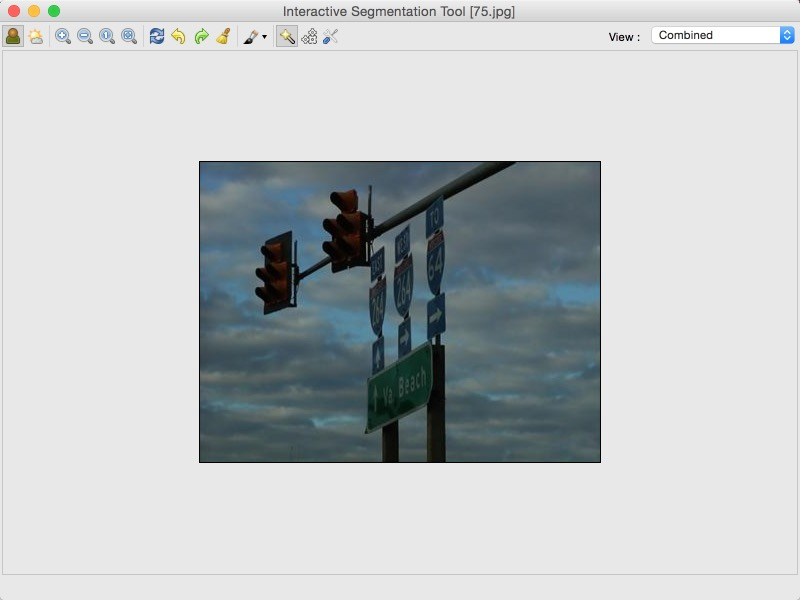
\includegraphics[width=0.5\columnwidth]{images/screenshot.png}
%\textbf{\caption{ The screenshot of k-space segmentation tool}}
%\label{fig:screenshot}
%\end{figure}

\subsection{User-interaction differences}
\paragraph{}In our person-oriented experiments, great differences among user labels were observed. It comes to us instinctively that different people tend to consider different part of foreground and background object as salient. Under this guidance, we processed the 5 label files of the same image and calculated the pair-wise intersection degree. The result is shown in Table \ref{ta:intersection degree f} and table \ref{ta:intersection degree b}. The intersection degree is defined as follows:
$$intersection\ of\ marked\ pixels/union\ of\ marked\ pixels$$
We make the following observations: (1)The mean value of intersection/union between every two people is quiet small, ranging from 1.6592\% to 3.5195\% in foreground and 0.0905\% to 0.9700\% in background, which indicates that labels made by different people have little in common. Figure \ref{fig:example} shows an example of user labels which share no common pixels (2) People share less similarities in background labels than foreground. It is mainly because the foreground objects are confined to a certain area while the backgrounds are more extensive.

\begin{table}
\parbox{.35\linewidth}{
\centering
\begin{tabular}{|c|c|c|c|c|c|}
\hline
 Label & label 1 & label 2 & label 3 & label 4& label 5 \\
\hline
label 1 & 100\% & 2.3768\% & 3.5195\% & 2.0146\%& 1.6592\% \\
\hline
label 2 & 2.3768\% & 100\% & 2.7080\% & 2.1684\%& 2.2459\% \\
\hline
label 3 & 3.5195\% & 2.7080\% & 100\% & 2.0485\%& 2.0102\%\\
\hline
label 4 & 2.0146\% & 2.1684\% & 2.0485\% & 100\%& 1.8441\% \\
\hline
label 5 & 1.6592\% & 2.2459\% & 2.0102\% & 1.8441\%& 100\% \\
\hline
\end{tabular}
\captionsetup{justification=centerlast}
\caption{intersection degree of foreground labels}
\label{ta:intersection degree f}
}
\hfill
\parbox{.35\linewidth}{
\centering
\begin{tabular}{|c|c|c|c|c|c|}
\hline
 Label & label 1 & label 2 & label 3 & label 4& label 5 \\
\hline
label 1 & 100\% & 0.8700\% & 0.8600\% & 0.0905\%& 0.6300\% \\
\hline
label 2 & 0.8700\% & 100\% & 0.9700\% & 0.2100\%& 0.7300\% \\
\hline
label 3 & 0.8600\% & 0.9700\% & 100\% & 0.1600\%& 0.6800\%\\
\hline
label 4 & 0.0905\% & 0.2100\% & 0.1600\% & 100\%& 0.6700\% \\
\hline
label 5 & 0.6300\% & 0.7300\% & 0.6800\% & 0.6700\% & 100\% \\
\hline
\end{tabular}
\captionsetup{justification=centerlast}
\caption{intersection degree of background labels}
\label{ta:intersection degree b}
}
\end{table}






\begin{figure}
\centering

\subfigure[source image] { \label{fig:a}
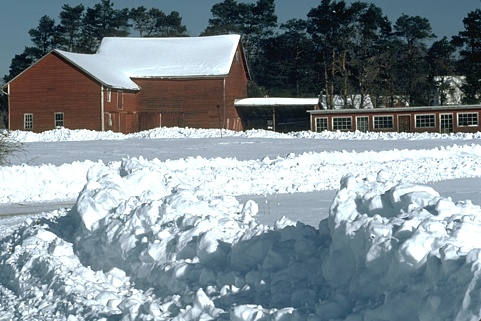
\includegraphics[width=0.2\columnwidth]{images/97033.jpg}
}
\subfigure[ground truth] { \label{fig:b}
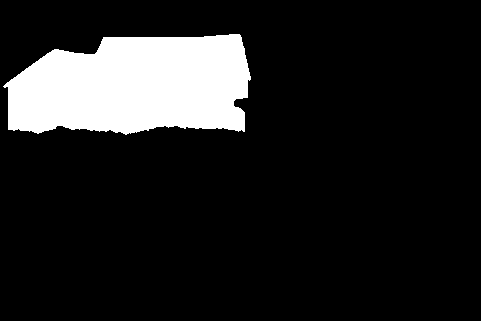
\includegraphics[width=0.2\columnwidth]{images/97033-gt.png}
}
\subfigure[label1] { \label{fig:c}
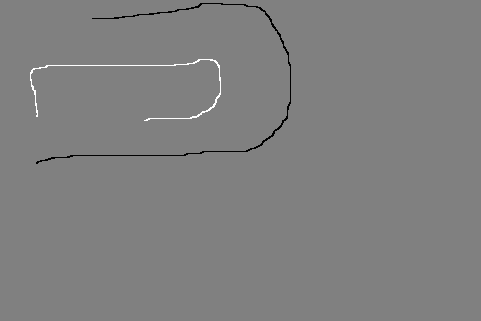
\includegraphics[width=0.2\columnwidth]{images/97033-5.png}
}
\subfigure[label2] { \label{fig:d}
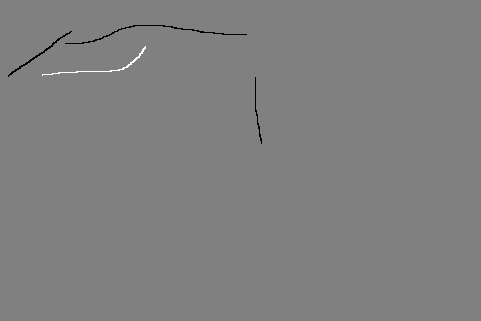
\includegraphics[width=0.2\columnwidth]{images/97033-4.png}
}
\subfigure[label example] { \label{fig:label example}
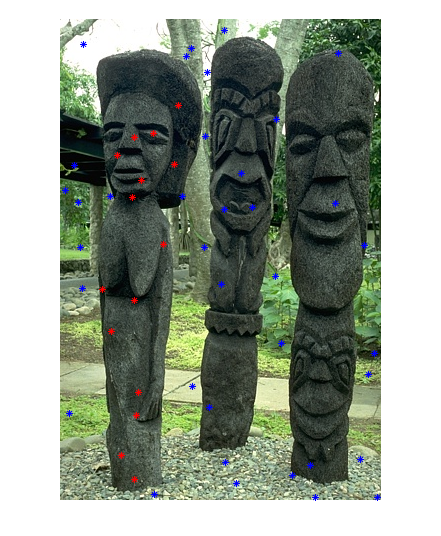
\includegraphics[width=0.5\columnwidth]{images/label-example2.png}
}
\caption{ Examples of user labels and auto-generated labels. (a) shows a source image, (b) shows the ground truth of image(a), (c)(d)shows two labels which show no common pixels. }
\label{fig:example}
\end{figure}


\subsection{Segmentation result difference}
\paragraph{}Based on the above result, we took a step further by examine the segmentation results of different labels.The implementation of four interactive segmentation algorithms in \citep{gulshan2010geodesic} was used. Based on the 96*5*4 segmentation results, we have found out that due to the variance between different labels, the segmentation results tend to be quite different, too.  We arrived here by calculating percent of pixels which was segmented out as foreground simultaneously by 1 person, two people, three people ,four people and 5 people out of all the segmented pixels. The result is shown in Table \ref{ta:bj intersection} \ref{ta:gsc intersection} \ref{ta:sp intersection} \ref{ta:rw intersection}. We have observed that: (1) The effectiveness of different labels as input of interactive segmentation algorithms vary from person to person, as could be observed that the label made by participant 1 have a better performance than others in terms of mean, maximum and minimum, which means there exists kind of "professional lables" \citep{fu2008saliency} (2) In mean level, the result reaches at most 66.760\% in table 5 made by participant 1. While the maximum ratio could be high as 99.050\%, the minimum ratio was also low as 1.060\%. This shows that when applied to segmentation algorithms, the variance of labels could further lead to even greater difference in segmentation results.

\begin{table}
\centering
\begin{tabular}{|c|c|}
\hline
Algorithm shorthand & Description\\
\hline
BJ\citep{boykov2001interactive} &  Boykov Jolly Graph cut  \\
\hline
GSC\citep{gulshan2010geodesic}& Boykov Jolly with Geodesic Star-Convexity \\
\hline
SP\citep{bai2007geodesic} & Bai and Sapiro \\
\hline
RW\citep {grady2006random}& Random Walker  \\
\hline
\end{tabular}
\caption{Interactive image segmentation algorithms}
\label{ta:algorithms}
\end{table}




\begin{table}
\centering
\begin{tabular}{|c|c|c|c|c|c|}
\hline
 intersection scale & 1 & 2 & 3 & 4& 5 \\
\hline
mean& 66.360\% & 55.090\% & 52.300\% & 50.710\%& 49.620\% \\
\hline
max& 99.020\% & 98.580\% & 98.370\% & 98.200\%& 98.060\% \\
\hline
min& 21.060\% & 1.240\% & 1.180\% & 1.160\%& 1.140\%\\
\hline
variance& 0.0557 & 0.0883 & 0.0897 & 0.0899& 0.0898 \\
\hline
coefficient of variance& 0.3556 & 0.5394 & 0.5727 & 0.5913& 0.6039\\
\hline
\end{tabular}
\caption{Segmentation intersection on algorithm BJ}
\label{ta:bj intersection}
\end{table}

\begin{table}
\centering
\begin{tabular}{|c|c|c|c|c|c|}
\hline
intersection scale & 1 & 2 & 3 & 4& 5 \\
\hline
mean& 66.760\% & 55.490\% & 52.490\% & 50.600\%& 49.170\% \\
\hline
max& 99.040\% & 98.500\% & 98.170\% & 97.900\%& 97.660\% \\
\hline
min& 21.130\% & 1.230\% & 1.100\% & 1.080\%& 1.060\%\\
\hline
variance& 0.0518 & 0.0809 & 0.0813 & 0.0812& 0.0812 \\
\hline
coefficient of variance& 0.3409 & 0.5126 & 0.5432 & 0.5632& 0.5795\\
\hline
\end{tabular}
\caption{Segmentation intersection on algorithm GSC}
\label{ta:gsc intersection}
\end{table}


\begin{table}
\centering
\begin{tabular}{|c|c|c|c|c|c|}
\hline
intersection scale & 1 & 2 & 3 & 4& 5 \\
\hline
mean& 56.390\% & 41.030\% & 36.740\% & 34.350\%& 32.660\% \\
\hline
max& 96.040\% & 94.290\% & 93.470\% & 92.850\%& 92.260\% \\
\hline
min& 22.950\% & 2.920\% & 2.270\% & 2.030\%& 1.910\%\\
\hline
variance& 0.0286 & 0.0431 & 0.0418& 0.0405&0.0393 \\
\hline
coefficient of variance& 0.2999 & 0.5060 & 0.5565 & 0.5859& 0.6070\\
\hline
\end{tabular}
\caption{Segmentation intersection on algorithm SP}
\label{ta:sp intersection}
\end{table}

\begin{table}
\centering
\begin{tabular}{|c|c|c|c|c|c|}
\hline
intersection scale & 1 & 2 & 3 & 4& 5 \\
\hline
mean& 63.180\% & 49.860\% & 45.720\% & 43.180\%& 41.410\% \\
\hline
max& 98.660\% & 97.910\% & 97.430\% & 97.010\%& 96.600\% \\
\hline
min& 23.010\% & 3.190\% & 2.580\% & 2.190\%& 2.000\%\\
\hline
variance& 0.0295 & 0.0440 & 0.0432 & 0.0433& 0.0436 \\
\hline
coefficient of variance& 0.2719 & 0.4207 & 0.4546 & 0.4819& 0.5042\\
\hline
\end{tabular}
\caption{Segmentation intersection on algorithm RW}
\label{ta:rw intersection}
\end{table}


\section{Semi-automatic Labelling Generation}

\subsection{Image representation for labelling quantitative analysis}
\paragraph{} In interactive image segmentation,users are expected labels some key features of the image foreground and background. The effectiveness of these labels is greatly related to their coverage of foreground and background key components. So we decide to simulate labels by simulating their coverage of key pixel clusters. In our method, we used the simple linear iterative clustering (SLIC)  method \citep{achanta2010slic} implemented by VLFeat open source library\citep{vedaldi08vlfeat}. The SLIC algorithm clusters pixels in the combined five-dimensional color and image plane space which brings compact, nearly uniform superpixels. We then decompose all the superpixels into distinct groups according to the quantitative rgb feature of each superpixel. In this way, we could analyze user labels on both superpixel level and superpixel group level.  On the level of superpixel, we are aimed at analyzing the amount of manual labour of providing certain labels; on the level of superpixel group, we could estimate the amount of information or key features provided by the labels.



\subsection{Effect of connection in labelling}
\paragraph{} Instead of continuous user scribbles, our simulation is planned to generating several points to represent key features in the image. So our first step was to validate the effectiveness of points in segmentation as compared to continuous lines. After figuring out the superpixel groups which were covered by user labels, we randomly select one superpixel from these groups and then randomly select one point from that superpixel. In this way, we formed a point set which contains points from groups covered by a certain human-made label. An example of our auto-generated label is shown in figure \ref{fig:example}.  We then apply five sets of this kind of labels to the four segmentation algorithms. In terms of evaluation of segmentation accuracy, we define the following criteria:

\begin{empheq}[box=\fbox]{align}
\begin{split}
 F_{gt} &= \text{foreground in ground truth}     \\
 F_{s}  &= \text{foreground in segmentation}     \\
  \text{recall}    &= \frac{F_{gt} \cap F_s}{F_{gt}}  \\
  \text{precision} &= \frac{F_{gt} \cap F_s}{F_{s}}  \\
  \end{split}
\end{empheq}


The accuracy evaluation of five batches of human-made labels and five batches of auto-generated labels applied to four algorithms are shown in Table  \ref{ta: simu in bj} \ref{ta: simu in gsc} \ref{ta: simu in sp} \ref{ta: simu in rw}. The precision and recall value are defined to be the mean value on all the images. We have observed that our simulated label points achieves a very similar precision and recall level as human labels do. This approves the validity of our assumption: discrete points which representing key features of the image could also act as effective labels. 
\begin{table}
\centering
\begin{tabular}{|c|c|c|c|c|c|}
\hline
 & label 1 & label 2&label 3&label 4&label 5 \\
\hline
Precision& 0.8595 & 0.8423 & 0.8449& 0.8543& 0.7474 \\
\hline
Recall& 0.8822 & 0.9158 & 0.9154& 0.9303& 0.9108 \\
\hline
 & simu-label 1 & simu-label 2&simu-label 3&simu-label 4&simu-label 5 \\
 \hline
Precision& 0.8659 & 0.8850 & 0.8500& 0.8327& 0.8997 \\
\hline
Recall& 0.8101 & 0.8339 & 0.8780& 0.8740& 0.8337  \\
\hline
\end{tabular}
\caption{BJ}
\label{ta: simu in bj}
\end{table} 


\begin{table}
\centering
\begin{tabular}{|c|c|c|c|c|c|}
\hline
 & label 1 & label 2&label 3&label 4&label 5 \\
  \hline
Precision& 0.8671 & 0.8619 & 0.8560& 0.8747& 0.7562 \\
\hline
Recall& 0.8794 & 0.9177 & 0.9137& 0.9183& 0.9129  \\
\hline
 & simu-label 1 & simu-label 2&simu-label 3&simu-label 4&simu-label 5 \\
\hline
Precision& 0.8885 & 0.8823 & 0.8733& 0.8443& 0.7856 \\
\hline
Recall& 0.8371 & 0.8366 & 0.8939& 0.8813& 0.8403 \\
\hline
\end{tabular}
\caption{GSC}
\label{ta: simu in gsc}
\end{table} 

\begin{table}
\centering
\begin{tabular}{|c|c|c|c|c|c|}
\hline
 & label 1 & label 2&label 3&label 4&label 5 \\
\hline
Precision& 0.6471 & 0.6567 & 0.6534& 0.7069& 0.6811 \\
\hline
Recall& 0.9306 & 0.9501 & 0.9454& 0.8991& 0.9015 \\
\hline
 & simu-label 1 & simu-label 2&simu-label 3&simu-label 4&simu-label 5 \\
\hline
Precision& 0.6722 & 0.6995 & 0.6802& 0.6631& 0.7153 \\
\hline
Recall& 0.9251 & 0.9221 & 0.9331& 0.9249& 0.9189 \\
\hline
\end{tabular}
\caption{SP}
\label{ta: simu in sp}
\end{table} 


\begin{table}
\centering
\begin{tabular}{|c|c|c|c|c|c|}
\hline
 & label 1 & label 2&label 3&label 4&label 5 \\
\hline
Precision& 0.7591 & 0.7672 & 0.7672& 0.8496& 0.7057 \\
\hline
Recall& 0.8837 & 0.9109 & 0.9019& 0.9279& 0.8759 \\
\hline
 & simu-label 1 & simu-label 2&simu-label 3&simu-label 4&simu-label 5 \\
\hline
Precision& 0.7716 & 0.7781 & 0.7556& 0.7716& 0.7766 \\
\hline
Recall& 0.8347 & 0.8477 & 0.8568& 0.8515& 0.8438 \\
\hline
\end{tabular}
\caption{RW}
\label{ta: simu in rw}
\end{table} 


\subsection{Solution space for labelling generation}
\paragraph{} In order to generate automatic labels, we need to figure out the consistence among labels made by different users. So we further analyzed the labels on both superpixel level and superpixel group level. Table \ref{ta: label coverage f} shows coverage rate of superpixel groups in foreground and Table \ref{ta: label coverage b} shows the situation in background.
We have observed that the maximum coverage reaches 100\% in every batch of labels and there exists low coverage in both foreground label and background label. Also, inside a single batch of labels which were made by the same user, the coverage rate is rather stable, as is indicated by low variance and coefficient of variance. 


\begin{table}
\centering
\begin{tabular}{|c|c|c|c|c|c|c|c|}
\hline
 & label 1 & label 2&label 3&label 4&label 5&mean&Variance\\
\hline
Mean& 74.9206\% & 81.9107\% & 83.5839\%& 83.1823\%& 76.5065\%&80.0208\%&0.0016 \\
\hline
Variance& 0.0265 & 0.0189 & 0.0211& 0.0235& 0.0277&NAN&NAN \\
\hline
CV& 0.2176 & 0.1680 & 0.1740& 0.1843& 0.2178&NAN&NAN \\
\hline
\end{tabular}
\caption{Superpixel group coverage in foreground.}
\label{ta: label coverage f}
\end{table} 

% CV: coefficient of variation
\begin{table}
\centering
\begin{tabular}{|c|c|c|c|c|c|c|c|c|c|c|}
\hline
 & label 1 & label 2&label 3&label 4&label 5&mean&Variance \\
\hline
Mean& 64.9213\% & 64.4634\% & 65.4448\%& 61.1484\%& 74.1032\%&66.0162\%&0.0023 \\
\hline
Variance& 0.0309 & 0.0191 & 0.0212& 0.0376& 0.0168&NAN&NAN \\
\hline
Coefficient of variance& 0.2709 & 0.2144 & 0.2227& 0.3170& 0.1747&NAN&NAN \\
\hline
\end{tabular}
\caption{Superpixel group coverage in background.}
\label{ta: label coverage b}
\end{table} 


\paragraph{} Based on the rather stable level of group coverage, we calculate the mean group overlap rate between every two labels on the same image. Table \ref{ta:group overlap f} and Table \ref{ta:group overlap b}  shows the value in foreground and background. Value in position (i,j) denotes the percent of groups in label i which were also covered in label j. We could note that the overlap rate between every two participants is rather high; We also examined the overlap rate on superpixel level. Table \ref{ta: sp overlap f} and Table \ref{ta: sp overlap b} shows the result. It is obvious that different users share little common ground on the superpixel level. 

\begin{table}
\parbox{.35\linewidth}{
\centering
\begin{tabular}{|c|c|c|c|c|c|c|c|}
\hline
 & label 1 & label 2&label 3&label 4&label 5&mean\\
\hline
label1& 100\% & 91.44\% & 92.86\%& 89.71\%& 88.64\%&90.66\%\\
\hline
label2& 83.86\% & 100\% & 90.75\%& 88.82\%& 85.93\%&87.34\%\\
\hline
label3& 83.40\% & 89.04\% & 100\%& 88.18\%& 84.62\%&86.31\% \\
\hline
label4& 80.75\% & 87.15\% & 88.15\%& 100\%& 82.44\%&84.62\% \\
\hline
label5& 82.53\% & 92.06\% & 92.10\%& 89.31\%& 100\%&90.00\% \\
\hline
\end{tabular}\captionsetup{justification=centerlast}
\caption{Group overlap between labels in foregorund}
\label{ta:group overlap f}
}
\hfill
\parbox{.35\linewidth}{
\centering
\begin{tabular}{|c|c|c|c|c|c|c|c|}
\hline
 & label 1 & label 2&label 3&label 4&label 5&mean\\
\hline
label1& 100\% &80.19\% & 81.61\%& 72.23\%& 86.97\%&80.25\%\\
\hline
label2& 80.22\% & 100\% & 82.65\%& 74.86\%& 88.57\%&81.58\% \\
\hline
label3& 80.25\% & 81.42\% & 100\%& 74.09\%& 88.36\%&81.03\%\\
\hline
label4& 77.40\% & 80.30\% & 80.15\%& 100\%& 88.78\%&81.66\% \\
\hline
label5& 76.36\% & 77.76\% & 78.21\%& 73.21\%& 100\%&76.39\%\\
\hline
\end{tabular}

\captionsetup{justification=centerlast}
\caption{Group overlap between labels in backgorund}
\label{ta:group overlap b}
}
\end{table}



\paragraph{}Based on analysis on superpixel and superpixel group level, we safely conclude that labels of different users are consistent on the defined superpixel group level but inconsistent on superpixel level. It is because certain key features of an image could be represented by different superpixels. Though there are limited number of key features of an object, users are sensitive to different representative superpixels. Also, the high level of superpixel group coverage( with the mean value arounf 85\%) and low level of superpixel coverage reveals two rules to us: (1) When labelling images, people are intended to provide as much information as possible(as indicated by the high coverage of superpixel groups)  (2) While aimed at labelling more key features, people also want to reduce the times of interaction or the total amount of labels, that is, shorter length within the same width. (as shown by the low coverage of superpixels)




\begin{table}
\parbox{.35\linewidth}{
\centering
\begin{tabular}{|c|c|c|c|c|c|c|}
\hline
 & label 1 & label 2&label 3&label 4&label 5&mean\\
\hline
label1& 100\% & 3.70\% & 3.69	\%& 3.39\%& 3.35\%& 3.53\%\\
\hline
label2& 2.91\% & 100\% & 3.32\%& 3.14\%& 3.00\% & 3.09\%\\
\hline
label3& 2.78\% & 3.23\% & 100\%& 2.93\%& 2.90\%& 2.96\% \\
\hline
label4& 2.24\% & 2.63\% & 2.55\%& 100\%& 2.37\%& 2.45\%\\
\hline
label5& 2.25\% & 2.56\% & 2.58\%& 2.45\%& 100\%& 2.46\% \\
\hline
\end{tabular}
\captionsetup{justification=centerlast}
\caption{superpixel overlap between labels in foreground}
\label{ta: sp overlap f}
}
\hfill
\parbox{.35\linewidth}{
\centering
\begin{tabular}{|c|c|c|c|c|c|c|}
\hline
 & label 1 & label 2&label 3&label 4&label 5&mean\\
\hline
label1& 100\% & 1.65\% & 1.59	\%& 0.49\%& 1.42\%& 1.29\%\\
\hline
label2& 1.70\% & 100\% & 5.33\%& 1.91\%& 1.81\%& 2.69\% \\
\hline
label3& 1.52\% & 1.75\% & 100\%& 0.65\%& 1.77\%& 1.42\% \\
\hline
label4& 0.39\% & 0.64\% & 0.59\%& 100\%& 1.56\%& 0.80\%\\
\hline
label5& 0.87\% & 1.08\% & 1.13\%& 1.18\%& 100\%& 1.07\% \\
\hline
\end{tabular}
\captionsetup{justification=centerlast}
\caption{superpixel overlap between labels in background}
\label{ta: sp overlap b}
}
\label{ta: sp overlap}
\end{table}




\subsection{Labelling generation}
\paragraph{} In labelling generation, we test the normality of superpixel coverage distribution and superpixel-group coverage distribution.The Normal Q-Q plot of the four coverage rate is shown in \ref{fig: qq plot}. As we can see from the plot below, the data points of four plots are all close to the diagonal line which indicates a normal distribution. We then fit the four distribution to normal distribution, as is shown in Figure \ref{fig:histogram} and figure out the probability distribution function of both superpixel coverage percent and superpixel group coverage percent as $coverage \sim \mathcal{N} (m,\sigma^2)$
\paragraph{} Then our labelling generation process is carried out as following: For each image (1) We first generate two coverage percent of superpixel and superpixel group according to the calculated  distribution. (2) Randomly select groups according to the target percentage. (3) Select superpixels in each group for labelling according to the size of the group and the overall percentage. 

\begin{figure}
\centering

\subfigure[Normal Q-Q plot of superpixel group coverage rate in foreground] { \label{fig:a2}
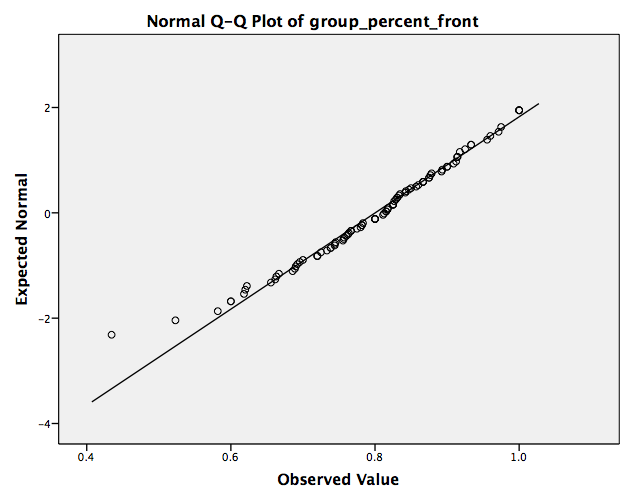
\includegraphics[width=0.4\columnwidth]{images/qq_group_f.png}
}
\subfigure[Normal Q-Q plot of superpixel group coverage rate in background] { \label{fig:b2}
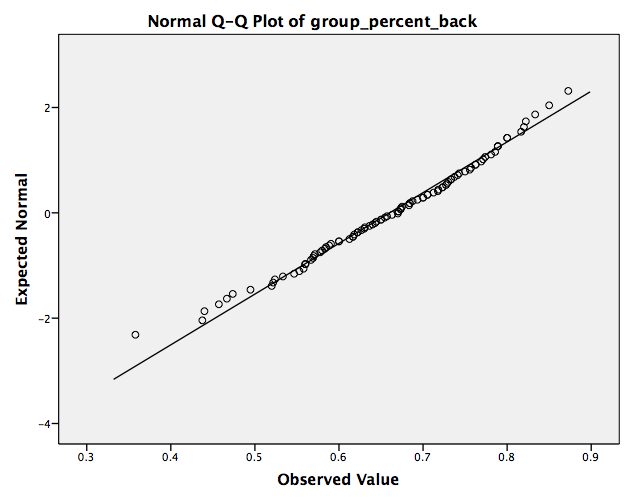
\includegraphics[width=0.4\columnwidth]{images/qq_group_b.png}
}
\subfigure[Normal Q-Q plot of superpixel coverage rate in foreground] { \label{fig:c}
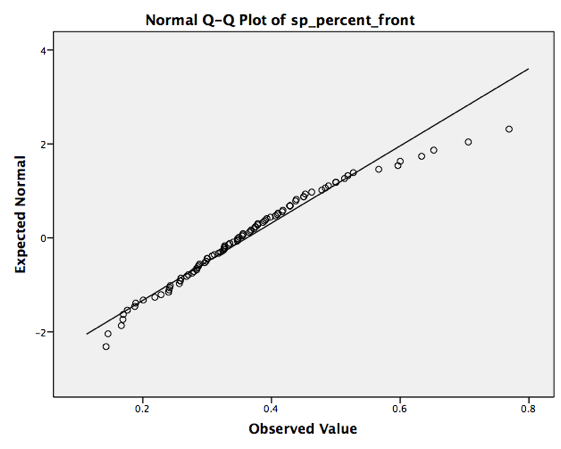
\includegraphics[width=0.4\columnwidth]{images/qq_sp_f.png}
}
\subfigure[Normal Q-Q plot of superpixel coverage rate in background] { \label{fig:c}
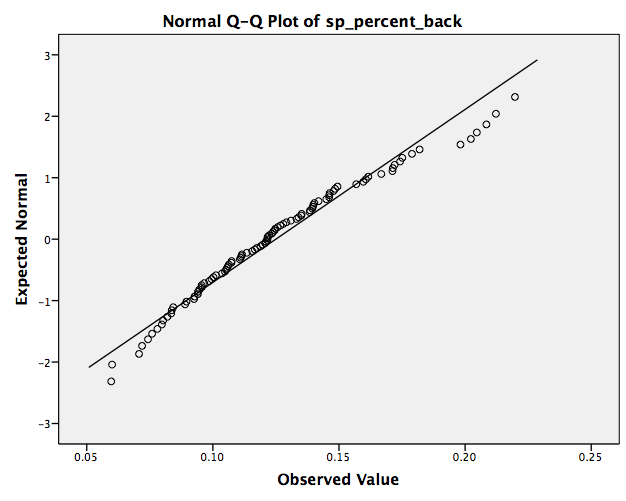
\includegraphics[width=0.4\columnwidth]{images/qq_sp_b.png}
}
\caption{ Probability distribution of superpixel group/ superpixel  }
\label{fig: qq plot}
\end{figure}


\begin{figure}
\centering

\subfigure[Distribution of superpixel group coverage rate in foreground ] { \label{fig:a2}
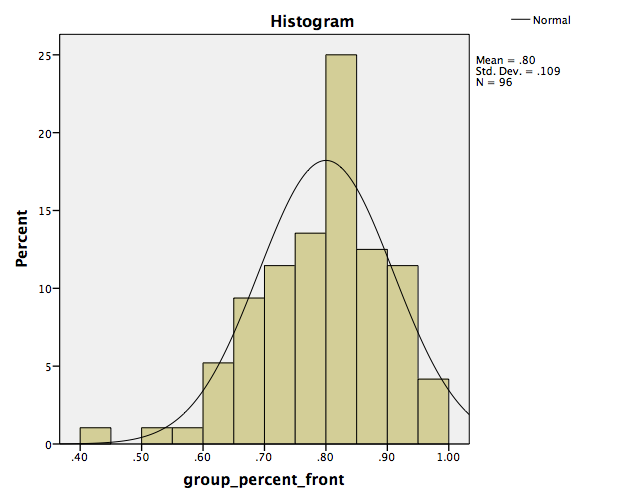
\includegraphics[width=0.4\columnwidth]{images/group_p_f.png}
}
\subfigure[Distribution of superpixel group coverage rate in background] { \label{fig:b2}
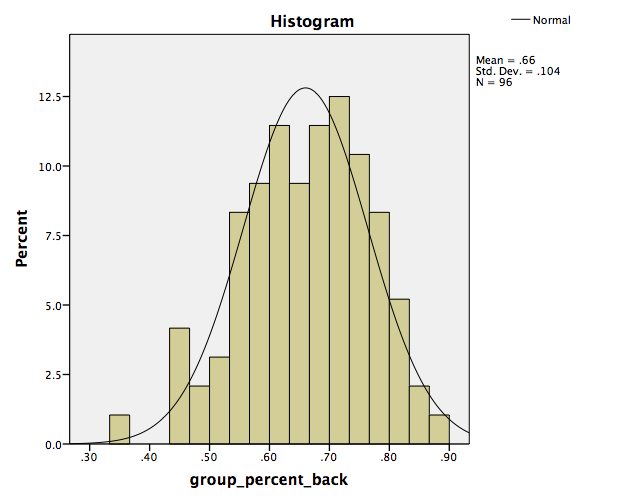
\includegraphics[width=0.4\columnwidth]{images/group_p_b.png}
}
\subfigure[Distribution of superpixel coverage rate in foreground] { \label{fig:c2}
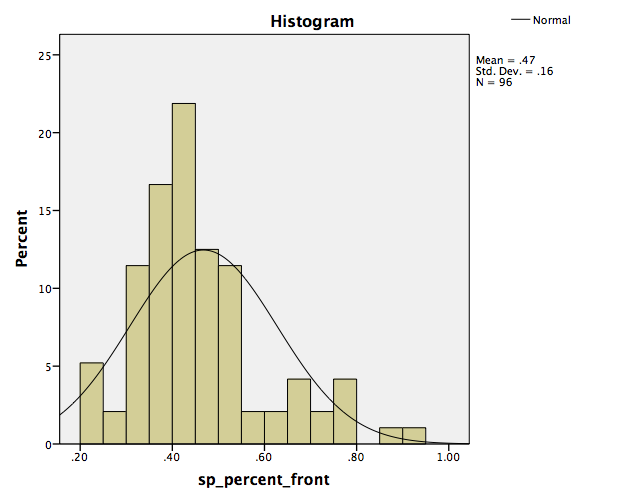
\includegraphics[width=0.4\columnwidth]{images/sp_p_f.png}
}
\subfigure[Distribution of superpixel coverage rate in background] { \label{fig:d2}
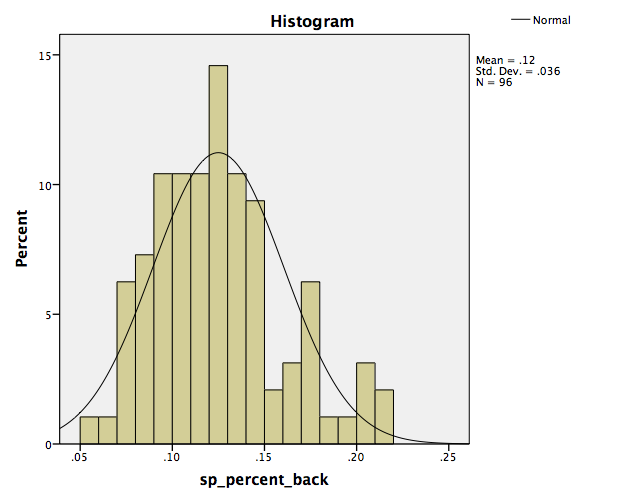
\includegraphics[width=0.4\columnwidth]{images/sp_p_b.png}
}
\caption{ Probability distribution of superpixel group/ superpixel  }
\label{fig:histogram}
\end{figure}



\section{Evaluation of Interactive Segmentation Algorithms}
We then test the four algorithms respectively with 96*5 auto-generated user labels and compare the result with the outcome of the previous 96*5 human-made labels. We also provide labels generated in the following ways for comparison: (1) Randomly select a superpixel in each superpixel group for labelling(all-group-2). (2) Randomly select certain percentage of superpixels among all superpixels without grouping them(all-group-1). 
The result is shown in figure \ref{fig:pr boxplot}. In each figure, the first two boxplots show the precision value of human-made labels and auto-generate labels while the following two boxplots show the recall value. 


We make the following observations: (1) The performance of four algorithms remains similar under our auto-generated labels (the second column) compared with human-made labels, which confirms the effectiveness of our simulation methods. (2) The thrid set of labels (the third column) are generated by cover all superpixel groups, thus providing more information than normal human labels could do, as could be indicated by its high precision value.(3) The fourth set of labels(the fourth column)  are generated randomly on all the superpixels. It shows the lowest precision level as it does not provide diverse information as superpixel groups could do.  (3) GSC \citep{gulshan2010geodesic} remains the best system on the whole dataset with high accuracy and stable performance. While RW \citep {grady2006random} and BJ \citep{boykov2001interactive}are expected to have similar performance, RW presents more robustness on both sets of labels. The SP\citep{bai2007geodesic} algorithm still achieves the poorest performance, mainly due to its lack of sensitivity to label locations.




\begin{figure}
\centering
\subfigure[Precision value of BJ with human-made and auto-generate labels] { \label{fig:a3}
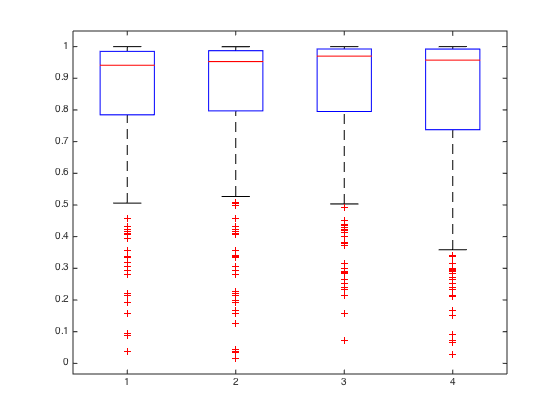
\includegraphics[width=0.4\columnwidth]{images/bj-eva-p.png}
}
\subfigure[Recall value of BJ with human-made and auto-generate labels] { \label{fig:b3}
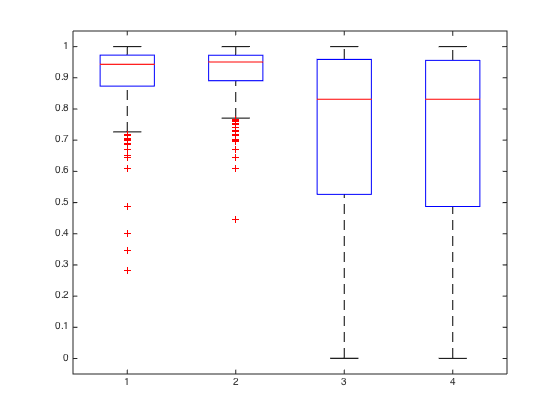
\includegraphics[width=0.4\columnwidth]{images/bj-eva-r.png}
}
\subfigure[Precision value of GSC with human-made and auto-generate labels] { \label{fig:c3}
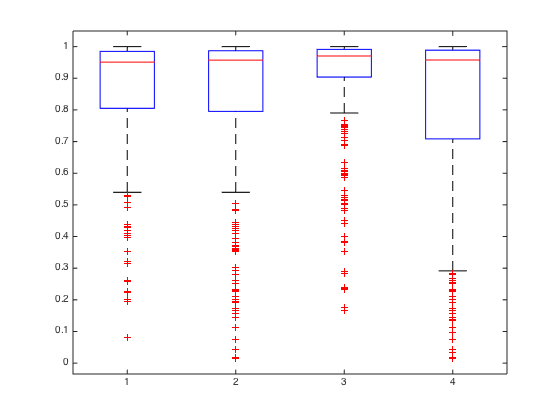
\includegraphics[width=0.4\columnwidth]{images/gsc-eva-p.png}
}
\subfigure[Recall value of GSC with human-made and auto-generate labels] { \label{fig:d3}
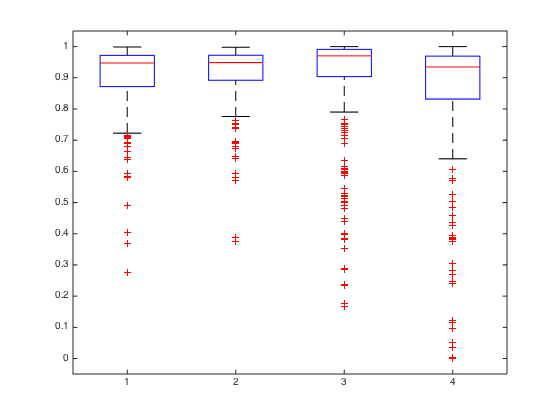
\includegraphics[width=0.4\columnwidth]{images/gsc-eva-r.png}
}
\subfigure[Precision value of RW with human-made and auto-generate labels] { \label{fig:e3}
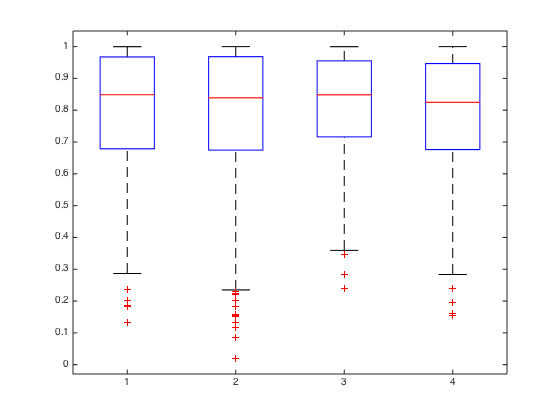
\includegraphics[width=0.4\columnwidth]{images/rw-eva-p.png}
}
\subfigure[Recall value of RW with human-made and auto-generate labels] { \label{fig:f3}
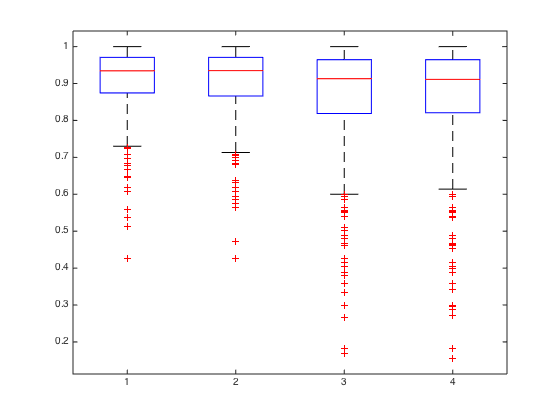
\includegraphics[width=0.4\columnwidth]{images/rw-eva-r.png}
}
\subfigure[Precision value of SP with human-made and auto-generate labels] { \label{fig:g3}
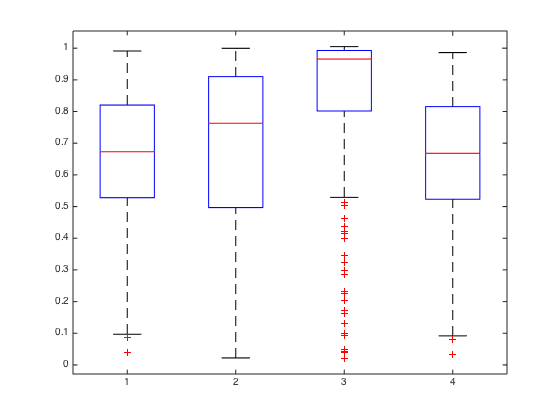
\includegraphics[width=0.4\columnwidth]{images/sp-eva-p.png}
}
\subfigure[Recall value of SP with human-made and auto-generate labels] { \label{fig:h3}
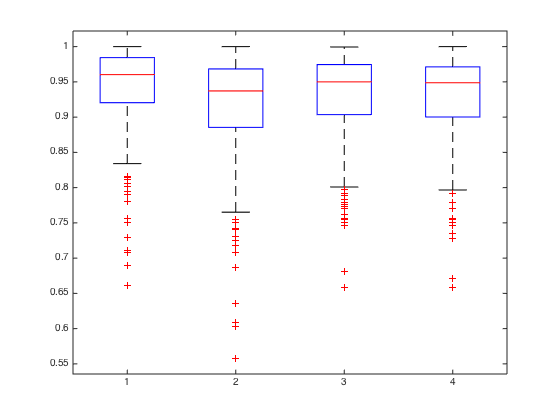
\includegraphics[width=0.4\columnwidth]{images/sp-eva-r.png}
}
\caption{Precision/recall value of four algorithms with human-made and auto-generated labels }
\label{fig:pr boxplot}
\end{figure}


\section{Conclusion}
In this paper, we propose a semi-automatic labelling generation method for evaluate interactive segmentation algorithms. We analyze the differences between multiple user labels and their segmentation results. Then we figure out the underlying consistence between user labels on the level of defined superpixel group. After validating the effectiveness of point-level simulation, a labelling simulation methodology is proposed to simulate user labels. Finally, four state-of-art algorithms are tested and evaluated by the auto-generated label.

\bibliographystyle{plain}
\bibliography{references}

%\end{thebibliography}



\end{document}
